\documentclass[12pt, a4paper]{article}

%<*preamble>
% Math symbols
\usepackage{amsmath, amsthm, amsfonts, amssymb}
\usepackage{accents}
\usepackage{esvect}
\usepackage{mathrsfs}
\usepackage{mathtools}
\mathtoolsset{showonlyrefs}
\usepackage{cmll}
\usepackage{stmaryrd}
\usepackage{physics}
\usepackage[normalem]{ulem}
\usepackage{ebproof}
\usepackage{extarrows}

% Page layout
\usepackage{geometry, a4wide, parskip, fancyhdr}

% Font, encoding, russian support
\usepackage[russian]{babel}
\usepackage[sb]{libertine}
\usepackage{xltxtra}

% Listings
\usepackage{listings}
\lstset{basicstyle=\ttfamily,breaklines=true}
\setmonofont[Scale=MatchLowercase]{JetBrains Mono}

% Miscellaneous
\usepackage{array}
\usepackage{booktabs}\renewcommand{\arraystretch}{1.2}
\usepackage{calc}
\usepackage{caption}
\usepackage{subcaption}
\captionsetup{justification=centering,margin=2cm}
\usepackage{catchfilebetweentags}
\usepackage{enumitem}
\usepackage{etoolbox}
\usepackage{float}
\usepackage{lastpage}
\usepackage{minted}
\usepackage{svg}
\usepackage{wrapfig}
\usepackage{xcolor}
\usepackage[makeroom]{cancel}

\newcolumntype{L}{>{$}l<{$}}
    \newcolumntype{C}{>{$}c<{$}}
\newcolumntype{R}{>{$}r<{$}}

% Footnotes
\usepackage[hang]{footmisc}
\setlength{\footnotemargin}{2mm}
\makeatletter
\def\blfootnote{\gdef\@thefnmark{}\@footnotetext}
\makeatother

% References
\usepackage{hyperref}
\hypersetup{
    colorlinks,
    linkcolor={blue!80!black},
    citecolor={blue!80!black},
    urlcolor={blue!80!black},
}

% tikz
\usepackage{tikz}
\usepackage{tikz-cd}
\usetikzlibrary{arrows.meta}
\usetikzlibrary{decorations.pathmorphing}
\usetikzlibrary{calc}
\usetikzlibrary{patterns}
\usepackage{pgfplots}
\pgfplotsset{width=10cm,compat=1.9}
\newcommand\irregularcircle[2]{% radius, irregularity
    \pgfextra {\pgfmathsetmacro\len{(#1)+rand*(#2)}}
    +(0:\len pt)
    \foreach \a in {10,20,...,350}{
            \pgfextra {\pgfmathsetmacro\len{(#1)+rand*(#2)}}
            -- +(\a:\len pt)
        } -- cycle
}

\providetoggle{useproofs}
\settoggle{useproofs}{false}

\pagestyle{fancy}
\lhead{Лабораторная работа №2}
\lfoot{Михайлов Максим}
\rfoot{M3337}
\cfoot{}
\rhead{стр. \thepage\ из \pageref*{LastPage}}

\newcommand{\R}{\mathbb{R}}
\newcommand{\Q}{\mathbb{Q}}
\newcommand{\Z}{\mathbb{Z}}
\newcommand{\B}{\mathbb{B}}
\newcommand{\N}{\mathbb{N}}
\renewcommand{\Re}{\mathfrak{R}}
\renewcommand{\Im}{\mathfrak{I}}

\newcommand{\const}{\text{const}}
\newcommand{\cond}{\text{cond}}

\newcommand{\teormin}{\textcolor{red}{!}\ }

\DeclareMathOperator*{\xor}{\oplus}
\DeclareMathOperator*{\equ}{\sim}
\DeclareMathOperator{\sign}{\text{sign}}
\DeclareMathOperator{\Sym}{\text{Sym}}
\DeclareMathOperator{\Asym}{\text{Asym}}

\DeclarePairedDelimiter{\ceil}{\lceil}{\rceil}

% godel
\newbox\gnBoxA
\newdimen\gnCornerHgt
\setbox\gnBoxA=\hbox{$\ulcorner$}
\global\gnCornerHgt=\ht\gnBoxA
\newdimen\gnArgHgt
\def\godel #1{%
    \setbox\gnBoxA=\hbox{$#1$}%
    \gnArgHgt=\ht\gnBoxA%
    \ifnum     \gnArgHgt<\gnCornerHgt \gnArgHgt=0pt%
    \else \advance \gnArgHgt by -\gnCornerHgt%
    \fi \raise\gnArgHgt\hbox{$\ulcorner$} \box\gnBoxA %
    \raise\gnArgHgt\hbox{$\urcorner$}}

% \theoremstyle{plain}

\theoremstyle{definition}
\newtheorem{theorem}{Теорема}
\newtheorem*{definition}{Определение}
\newtheorem{axiom}{Аксиома}
\newtheorem*{axiom*}{Аксиома}
\newtheorem{lemma}{Лемма}
\newenvironment{solution}[1][Решение.]{\begin{proof}[#1]}{\end{proof}}

\theoremstyle{remark}
\newtheorem*{remark}{Примечание}
\newtheorem*{exercise}{Упражнение}
\newtheorem{corollary}{Следствие}[theorem]
\newtheorem*{statement}{Утверждение}
\newtheorem*{corollary*}{Следствие}
\newtheorem*{example}{Пример}
\newtheorem{observation}{Наблюдение}
\newtheorem*{prop}{Свойства}
\newtheorem*{obozn}{Обозначение}

% subtheorem
\makeatletter
\newenvironment{subtheorem}[1]{%
    \def\subtheoremcounter{#1}%
    \refstepcounter{#1}%
    \protected@edef\theparentnumber{\csname the#1\endcsname}%
    \setcounter{parentnumber}{\value{#1}}%
    \setcounter{#1}{0}%
    \expandafter\def\csname the#1\endcsname{\theparentnumber.\Alph{#1}}%
    \ignorespaces
}{%
    \setcounter{\subtheoremcounter}{\value{parentnumber}}%
    \ignorespacesafterend
}
\makeatother
\newcounter{parentnumber}

\newtheorem{manualtheoreminner}{Теорема}
\newenvironment{manualtheorem}[1]{%
    \renewcommand\themanualtheoreminner{#1}%
    \manualtheoreminner
}{\endmanualtheoreminner}

\newcommand{\dbltilde}[1]{\accentset{\approx}{#1}}
\newcommand{\intt}{\int\!}

% magical thing that fixes paragraphs
\makeatletter
\patchcmd{\CatchFBT@Fin@l}{\endlinechar\m@ne}{}
{}{\typeout{Unsuccessful patch!}}
\makeatother

\newcommand{\get}[2]{
    \ExecuteMetaData[#1]{#2}
}

\newcommand{\getproof}[2]{
    \iftoggle{useproofs}{\ExecuteMetaData[#1]{#2proof}}{}
}

\newcommand{\getwithproof}[2]{
    \get{#1}{#2}
    \getproof{#1}{#2}
}

\newcommand{\import}[3]{
    \subsection{#1}
    \getwithproof{#2}{#3}
}

\newcommand{\given}[1]{
    Дано выше. (\ref{#1}, стр. \pageref{#1})
}

\renewcommand{\ker}{\text{Ker }}
\newcommand{\im}{\text{Im }}
\renewcommand{\grad}{\text{grad}}
\newcommand{\rg}{\text{rg}}
\newcommand{\defeq}{\stackrel{\text{def}}{=}}
\newcommand{\defeqfor}[1]{\stackrel{\text{def } #1}{=}}
\newcommand{\itemfix}{\leavevmode\makeatletter\makeatother}
\newcommand{\?}{\textcolor{red}{???}}
\renewcommand{\emptyset}{\varnothing}
\newcommand{\longarrow}[1]{\xRightarrow[#1]{\qquad}}
\DeclareMathOperator*{\esup}{\text{ess sup}}
\newcommand\smallO{
    \mathchoice
    {{\scriptstyle\mathcal{O}}}% \displaystyle
    {{\scriptstyle\mathcal{O}}}% \textstyle
    {{\scriptscriptstyle\mathcal{O}}}% \scriptstyle
    {\scalebox{.6}{$\scriptscriptstyle\mathcal{O}$}}%\scriptscriptstyle
}
\renewcommand{\div}{\text{div}\ }
\newcommand{\rot}{\text{rot}\ }
\newcommand{\cov}{\text{cov}}

\makeatletter
\newcommand{\oplabel}[1]{\refstepcounter{equation}(\theequation\ltx@label{#1})}
\makeatother

\newcommand{\symref}[2]{\stackrel{\oplabel{#1}}{#2}}
\newcommand{\symrefeq}[1]{\symref{#1}{=}}

% xrightrightarrows
\makeatletter
\newcommand*{\relrelbarsep}{.386ex}
\newcommand*{\relrelbar}{%
    \mathrel{%
        \mathpalette\@relrelbar\relrelbarsep
    }%
}
\newcommand*{\@relrelbar}[2]{%
    \raise#2\hbox to 0pt{$\m@th#1\relbar$\hss}%
    \lower#2\hbox{$\m@th#1\relbar$}%
}
\providecommand*{\rightrightarrowsfill@}{%
    \arrowfill@\relrelbar\relrelbar\rightrightarrows
}
\providecommand*{\leftleftarrowsfill@}{%
    \arrowfill@\leftleftarrows\relrelbar\relrelbar
}
\providecommand*{\xrightrightarrows}[2][]{%
    \ext@arrow 0359\rightrightarrowsfill@{#1}{#2}%
}
\providecommand*{\xleftleftarrows}[2][]{%
    \ext@arrow 3095\leftleftarrowsfill@{#1}{#2}%
}

\allowdisplaybreaks

\newcommand{\unfinished}{\textcolor{red}{Не дописано}}

% Reproducible pdf builds 
\special{pdf:trailerid [
<00112233445566778899aabbccddeeff>
<00112233445566778899aabbccddeeff>
]}
%</preamble>


\lhead{Домашнее задание №1}
\lfoot{Михайлов Максим}
\cfoot{}
\rfoot{M3237}

\begin{document}

\section{$2x^2yy'+y^2=2$}

\begin{align*}
    y'                            & =\frac{2-y^2}{2x^2y}               \\[1em]
    \frac{dy}{dx}                 & = \frac{2-y^2}{2x^2y}              \\[1em]
    \frac{ydy}{dx}                & = \frac{2-y^2}{2x^2}               \\[1em]
    \frac{ydy}{2-y^2}             & = \frac{dx}{2x^2}                  \\[1em]
    \int \frac{ydy}{2-y^2}        & = \int \frac{dx}{2x^2}             \\[1em]
    \int \frac{ydy}{2-y^2}        & = -\frac{1}{2x}                    \\[1em]
    t:                            & =2-y^2                             \\[1em]
    \int \frac{1}{2}\frac{-dt}{t} & = -\frac{1}{2x}                    \\[1em]
    -\frac{1}{2}\ln|2-y^2|        & = -\frac{1}{2x} + C                \\[1em]
    \ln|2-y^2|                    & =\frac{1}{x} + C                   \\[1em]
    |2-y^2|                       & = e^{\frac{1}{x} + C}              \\[1em]
    2-y^2                         & = \pm A e^{\frac{1}{x}}            \\[1em]
    2-y^2                         & = A e^{\frac{1}{x}}                \\[1em]
    y^2                           & = \pm (-A e^{\frac{1}{x}} + 2)     \\[1em]
    \text{Ответ: } y              & = \pm\sqrt{-A e^{\frac{1}{x}} + 2}
\end{align*}

\section{$y'=\cos(y-x)$}

Особое решение: $y = x + 2\pi n$

\begin{align*}
    \frac{dy}{dx}                                                           & =\cos(y-x)                             \\
    \frac{dy-dx+dx}{dx}                                                     & =\cos(y-x)                             \\
    \frac{dy-dx}{dx}+1                                                      & =\cos(y-x)                             \\
    t :                                                                     & = y-x                                  \\
    \frac{dy-dx}{dx}+1                                                      & =\cos(y-x)                             \\
    \frac{dt}{dx} + 1                                                       & = \cos(t)                              \\
    dt + dx                                                                 & = dx\cos(t)                            \\
    dt                                                                      & = dx(\cos(t) - 1)                      \\
    \frac{dt}{\cos(t) - 1}                                                  & = dx                                   \\
    \int\frac{dt}{\cos(t) - 1}                                              & = \int dx                              \\
    \int\frac{dt}{\cos(t) - 1}                                              & = x + C                                \\
    \bigintsss\frac{dt}{\cfrac{1-\tg^2\frac{t}{2}}{1+\tg^2\frac{t}{2}} - 1} & = x + C                                \\
    \int\frac{1+\tg^2\frac{t}{2}}{-2\tg^2\frac{t}{2}}dt                     & = x + C                                \\
    \int\frac{1}{-2\cos\frac{t}{2}\tg^2\frac{t}{2}}dt                       & = x + C                                \\
    a : = \tg\frac{t}{2}                                                    & \quad da = \frac{dt}{2\cos\frac{t}{2}} \\
    \int\frac{1}{-a^2}da                                                    & = x + C                                \\
    \frac{1}{a}                                                             & = x + C                                \\
    \frac{1}{\tg\frac{t}{2}}                                                & = x + C                                \\
    \frac{1}{\tg\frac{y-x}{2}}                                              & = x + C                                \\
    \arctg\frac{1}{x + C}                                                   & = \frac{y-x}{2} + \pi n, n\in\Z        \\
\end{align*}

Ответ: $y = 2\arctg\frac{1}{x + C} + x + 2\pi n$ или $y = x + 2\pi n, n\in \Z$

% \pagebreak

\section{$y'-y=2x-3$}

\begin{align*}
    \frac{dy}{dx} - y                                 & = 2x-3                                  \\
    \frac{dy}{dx}                                     & = 2x + y -3                             \\
    t := 2x + y                                       & \quad \frac{dt}{dx} = 2 + \frac{dy}{dx} \\
    \frac{dt}{dx} - 2                                 & = t - 3                                 \\
    \frac{dt}{dx}                                     & = t - 1                                 \\
    \frac{dt}{dx}                                     & = t - 1 \quad (*)                       \\
    \frac{dt}{t - 1}                                  & =  dx                                   \\
    \int \frac{dt}{t - 1}                             & = \int dx                               \\
    \ln(t - 1)                                        & = x + C                                 \\
    t-1                                               & = e^{x + C}                             \\
    2x+y-1                                            & = e^{x + C}                             \\
    (*): \sphericalangle t=1 \Leftrightarrow 2x+y = 1 & \text{ --- подходит}                    \\
\end{align*}
Ответ: $y = e^{x + C} + 1 - 2x$ или $y = 1 - 2x$

\section{$y'=\sqrt{4x+2y-1}$}

\begin{align*}
    \frac{dy}{dx}                     & = \sqrt{4x + 2y - 1}                     \\
    t := 4x + 2y                      & \quad \frac{dt}{dx} = 4 + 2\frac{dy}{dx} \\
    \frac{1}{2}\frac{dt}{dx} - 2      & = \sqrt{t - 1}                           \\
    \frac{dt}{dx}                     & = 2\sqrt{t - 1} + 4                      \\
    \frac{dt}{2\sqrt{t - 1} + 4}      & = dx                                     \\
    \int \frac{dt}{2\sqrt{t - 1} + 4} & = \int dx                                \\
    \int \frac{dt}{2\sqrt{t - 1} + 4} & = x + C                                  \\
    a := \sqrt{t - 1}                 & \quad da = \frac{dt}{2\sqrt{t-1}}        \\
    \int \frac{2ada}{2a + 4}          & = x + C                                  \\
\end{align*}

\begin{align*}
    \int \frac{ada}{a + 2}                           & = x + C \\
    \int \left(1 - \frac{2}{a + 2}\right)da          & = x + C \\
    a - \int \frac{2}{a + 2}  da                     & = x + C \\
    a - 2 \ln(a+2)                                   & = x + C \\
    \sqrt{t - 1} - 2 \ln(\sqrt{t - 1}+2)             & = x + C \\
    \sqrt{4x + 2y - 1} - 2 \ln(\sqrt{4x + 2y - 1}+2) & = x + C \\
\end{align*}

Дальше не решается :(, но вроде дальше и не надо.

\section{$x^2y'-\cos(2y) = 1,\ \ y(+\infty)=\frac{9\pi}{4}$}

\begin{align*}
    x^2\frac{dy}{dx} - \cos(2y)                                     & = 1                                            \\
    \frac{dy}{dx}                                                   & = \frac{1 + \cos(2y)}{x^2}                     \\
    \frac{dy}{1 + \cos(2y)}                                         & = \frac{dx}{x^2}                               \\
    \int \frac{dy}{1 + \cos(2y)}                                    & = \int \frac{dx}{x^2}                          \\
    \int \frac{dy}{1 + \cos(2y)}                                    & = - \frac{1}{x} + C                            \\
    \int \frac{dy}{1 + \frac{1-\tg^2 y}{1+\tg^2 y}}                 & = - \frac{1}{x} + C                            \\
    \int \frac{1+\tg^2 y}{2}dy                                      & = - \frac{1}{x} + C                            \\
    \frac{y}{2} + \int \frac{\frac{1}{\cos^2 y} - 1}{2}dy           & = - \frac{1}{x} + C                            \\
    \int \frac{1}{2\cos^2 y}dy                                      & = - \frac{1}{x} + C                            \\
    \frac{\tg y}{2}                                                 & = - \frac{1}{x} + C                            \\
    \tg y                                                           & = - \frac{2}{x} + A                            \\
    y                                                               & = \arctg\left(- \frac{2}{x} + A\right) + \pi n \\
    \lim_{x\to+\infty} y                                            & = \frac{9\pi}{4}                               \\
    \lim_{x\to+\infty} \arctg\left(- \frac{2}{x} + A\right) + \pi n & = \frac{9\pi}{4}                               \\
\end{align*}
\begin{align*}
    \arctg A + \pi n & = \frac{9\pi}{4}  \Rightarrow n = 2                     \\
    \arctg A         & = \frac{\pi}{4}                                         \\
    A                & = 1 + \pi k                                             \\
    \text{Ответ: } y & = \arctg\left(- \frac{2}{x} + 1 \right) + 2\pi,\ k\in\Z
\end{align*}

\section{$3y^2y'+16x=2xy^3, y(x)$ огр. при $x\to+\infty$}

\begin{align*}
    3y^2\frac{dy}{dx} + 16 x                                     & = 2xy^3                       \\
    3y^2\frac{dy}{dx}                                            & = 2xy^3 - 16 x                \\
    3y^2\frac{dy}{dx}                                            & = 2x(y^3 - 8)   (*)           \\
    \frac{3y^2}{(y^3 - 8)}dy                                     & = 2xdx                        \\
    \int \frac{3y^2}{y^3 - 8}dy                                  & = \int 2xdx                   \\
    \int \frac{3y^2}{y^3 - 8}dy                                  & = 4x^2 + C                    \\
    t := y^3                                                     & \quad dt = 3y^2dy             \\
    \int \frac{dt}{t - 8}                                        & = 4x^2 + C                    \\
    \ln(y^3 - 8)                                                 & = 4x^2 + C                    \\
    y^3 - 8                                                      & = e^{4x^2 + C}                \\
    y                                                            & = \sqrt[3]{e^{4x^2 + C} + 8}  \\
    \lim_{x\to+\infty} y                                         & \in\R                         \\
    \lim_{x\to+\infty} \sqrt[3]{e^{4x^2 + C} + 8}                & \in\R                         \\
    \lim_{x\to+\infty} e^{4x^2 + C}                              & = \infty                      \\
    (*): \sphericalangle y = 2 \Rightarrow 12y' = 0\Rightarrow y & \equiv 2 \text{ --- подходит} \\
    \text{Ответ: } y \equiv 2
\end{align*}

\section{Найти кривые, для которых площадь треугольника, образованного касательной, ординатой точки касания и осью абсцисс, есть величина постоянная, равная $a^2$}

Точки касания --- $x, y$, точка пересечения оси абсцисс и касательной --- $(x - \frac{y}{y'}, 0)$

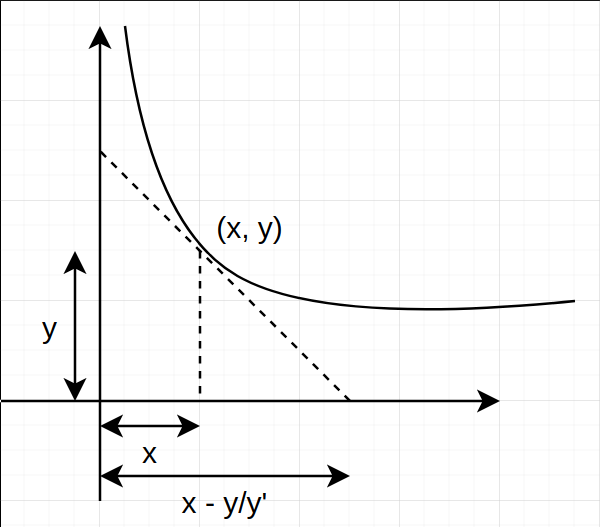
\includegraphics[scale=0.4]{images/1.6.png}

\begin{align*}
    a^2                  & = \frac{y \left(x - \frac{y}{y'} - x\right)}{2} \\
    a^2                  & = -\frac{y^2}{2y'}                              \\
    \frac{2y'}{y^2}      & = -\frac{1}{a^2}                                \\
    \int \frac{2dy}{y^2} & = \int -\frac{dx}{a^2}                          \\
    \frac{-2}{y}         & = -\frac{x}{a^2} + C                            \\
    \frac{2}{y}          & = \frac{x + A}{a^2}                             \\
    y                    & =    \frac{2a^2}{x + A}                         \\
\end{align*}

Для $y'>0$ точка пересечения оси абсцисс и касательной --- $(x + \frac{y}{y'}, 0)$, поэтому ответ $y=\frac{2a^2}{\pm x + A}$

\section{Найти кривые, касательные к которым в любой точке образуют равные углы с полярным радиусом и полярной осью.}

\subsection{Кривые в 1 или 4 квадранте}

Пусть угол в точке касания (\textit{между радиусом и осью}) --- $\alpha$, тогда по условию угол между касательной и осью $\cfrac{\pi - \alpha}{2}$

\begin{align*}
    \tg \frac{\pi - \alpha}{2}  & = \frac{r}{r'}                                      \\
    \tg \frac{\pi - \alpha}{2}  & = \frac{rd\alpha}{dr}                               \\
    \frac{dr}{r}                & = \ctg \frac{\pi - \alpha}{2} d\alpha               \\
    \int \frac{dr}{r}           & = \int \ctg \frac{\pi - \alpha}{2} d\alpha          \\
    \ln |r|                     & = \int \ctg \frac{\pi - \alpha}{2} d\alpha          \\
    t := \frac{\pi - \alpha}{2} & \quad dt = \frac{-d\alpha}{2}                       \\
    \ln |r|                     & = -2\int \ctg t dt                                  \\
    \ln |r|                     & = -2\ln\left|\sin t\right| + C                      \\
    \ln r                       & = -2\ln\left|\sin \frac{\pi - \alpha}{2}\right| + C \\
    r                           & = \sin^{-2} \left(\frac{\pi - \alpha}{2}\right) C_1 \\
    r                           & = \cos^{-2} \left(\frac{\alpha}{2}\right) C_1       \\
    r                           & = \frac{C_1}{\cos \alpha + 1}                       \\
\end{align*}

\subsection{Кривые в 2 или 3 квадранте}

Пусть угол в точке касания (\textit{между радиусом и осью}) --- $\alpha$, тогда по условию угол между касательной и осью $\cfrac{\alpha}{2}$

\begin{align*}
    \ln |r| & = \int \ctg \left(\frac{\alpha}{2}\right) d\alpha \\
    \ln |r| & = -2\ln\left|\sin t\right| + C                    \\
    r       & = \sin^{-2} \left(\frac{\alpha}{2}\right) e^C     \\
\end{align*}

Получается такая же кривая.

\section{Количество света, поглощаемое слоем воды малой толщины, пропорционально количеству падающего на него света и толщине слоя. Слой толщиной 35 см поглощает половину падающего на него света. Какую часть света поглотит слой воды 2 м?}

$\sphericalangle n$ --- поглощенная часть света

\begin{align*}
    n'           & = kn     \\
    dn           & = kndh   \\
    \frac{dn}{n} & = kdh    \\
    \ln n        & = kh + C \\
    n            & = e^{kh} \\
\end{align*}

$h = 0.35$ м, $n = \frac{1}{2}$:

\begin{align*}
    \frac{1}{2}         & = e^{k\cdot 0.35} \\
    \frac{1}{2}         & = e^{k\cdot 0.35} \\
    -\ln 2              & = k\cdot 0.35     \\
    \frac{-\ln 2}{0.35} & = k               \\
\end{align*}
Найдём искомое:
\begin{align*}
    n              & = e^{2k}                                    \\
    n              & = e^{\cfrac{-2\ln 2}{0.35}}                 \\
    n              & = e^{\cfrac{-40\ln 2}{7}}                   \\
    n              & = \left(\frac{1}{2}\right)^{\frac{40}{7}}   \\
    \text{Ответ: } & 1 - \left(\frac{1}{2}\right)^{\frac{40}{7}}
\end{align*}

\section{Резиновый шнур длиной в 1 м под действием силы $f$ удлиняется на $kf$ метров. На сколько удлинится такой же шнур длины $l$ и веса $P$ под действием своего веса, если подвесить за один конец?}

Сила, действующая на участок шнура длиной $dx$ на расстоянии $x$ от точки подвеса: $$F(x)=(l-x)\frac{P}{l} dx$$

\begin{align*}
    \int_0^l k F(x) dx & = \int_0^l k (l-x)\frac{P}{l} dx \\
                       & = \frac{Pk}{l} \frac{l^2}{2}     \\
                       & = \frac{Pkl}{2}                  \\
\end{align*}

Помогите Даше-путешественнице найти в этой задаче дифур.

\section{Масса ракеты с полным запасом топлива равна M, без топлива m, скорость истечения продуктов горения из ракеты равна c, начальная скорость ракеты равна нулю. Найти скорость ракеты после сгорания топлива, пренебрегая силой тяжести и сопротивлением воздуха.}

Пусть топлива истекло $a(t)$ (по массе) в момент времени $t$

Сохранение импульса:
\begin{align*}
    c da                  & = dv(M-a)           \\
    \frac{da}{(M-a)}      & = \frac{dv}{c}      \\
    \int \frac{da}{(M-a)} & = \int \frac{dv}{c} \\
    -\ln(M-a)             & = \frac{v}{c} + C   \\
    -c\ln(M-a) - C        & = v                 \\
\end{align*}
$v_0 = 0, a_0 = 0$:
\begin{align*}
    0 & = -c\ln(M) - C \\
    C & = -c\ln (M)    \\
\end{align*}

После сгорания топлива $a = M-m$

\begin{align*}
    v                & = -c\ln(M-M+m) + c\ln M        \\
    \text{Ответ: } v & = c\left(\ln\frac{M}{m}\right)
\end{align*}

\end{document}